\section{Введение}
Цифровое изображение имеет конечное количество пикселей. Количество этих пикселей деленное на единицу площади называется
разрешением цифрового изображения.

Для анализа и обработки изображений в большинстве случаев используются изображения высокого разрешения, так как они
позволяют увидеть детали, которые не различимы, или плохо различимы на изображениях с низким разрешением. Многие задачи
компьютерного зрения изначально полагаются на то, что изображение на входе в хорошем разрешение. Например, алгоритмы
распознавания автомобильного номера будут работать намного устойчивее, если на вход они будут получать изображение с
высоким разрешением. С первого взгляда,
задача увеличения разрешения чисто аппаратная -- чтобы увеличить разрешение необходимо просто взять фотоаппарат с
большей разрешающей способностью. Но часто уже имеется некоторая фотография или набор фотографий, и нет возможности
повторно произвести съемку. Примером может послужить низкокачественные картинки с изображений камер наблюдения. В этом
случае уместно использовать программные алгоритмы повышения разрешения (Super-resolution методы).  Эти алгоритмы
используют некоторое дополнительное знание о изображении для качественного повышения разрешения. Примером
дополнительных знаний может послужить информация о том, как двигался объект во время съемки, или оптические параметры
камеры. Зная эти параметры можно алгоритмическим путем получить более качественное изображение.

В этой работе рассмотрены два алгоритма для повышения разрешения на примере автомобильных номеров.

\section{Обзор существующих алгоритмов} Классические алгоритмы Super-Resolution делятся на четыре
категории\footnote{Стоит заметить, что существуют алгоритмы, которые будут плохо ложиться на эти категории. Но такие
алгоритмы не сыскали большой известности, поэтому из рассмотрения убраны.}.  Существует несколько обзорных статей по
этим алгоритмам \cite{ParkS.C.2003,tian2011survey}

\subsection{Обучаемые алгоритмы}
Обучаемые алгоритмы используют для восстановления изображений используют знание о том, что в действительности изображено
на картинке. Такие алгоритмы хорошо подходят для повышения разрешения однотипных изображений, таких как лица или
автомобильные номера.

\subsection{Интерполяционные} Подход интерполяции наиболее интуитивно понятный метод решения задачи SR. Решение задачи,
в общем случае, разбивается на три шага: определение относительного движения (Motion estimation) для каждого
изображения, интерполяция LR изображений на HR сетку, удаление смазывания и шума для полученного HR изображения.

\subsubsection{Метод ближайшего соседа}
При печати этого текста компьютером тоже была решена задача повышения разрешения, т.к. принтер печатает изображения с
намного более большим разрешением, чем была исходная картинка. В этом случае, задача решается не самым лучшим образом -
компьютер просто просчитывает недостающие точки используя значения пикселя изображения, который находится ближе всего.
Такая примитивная интерполяция называется <<метод ближайшего соседа>>.

\subsubsection{Билинейная интерполяция}
Билинейная интерполяция чуть более продвинутый метод интерполяции. Для интерполяции используется взвешенные суммы
линейных интерполяций по вертикальной и горизонтальной оси. Более подробное описание и формулу билинейной интерполяции
можно найти в \cite[стр. 64]{gonzalez2002woods}.

\subsubsection{Бикубическая интерполяция}
Бикубическая интерполяция обладает одним из лучших сочетаний качества и скорости.  Бикубическая
интерполяция являеется обобщением интерполяции кубическими сплайнами на двумерный случай. Алгоритм кубической
интерполяции реализован во многих редакторах цифровых изображений. В нашей статье мы будем считать алгоритм бикубической
интерполяции отправной точкой. По сравнение результатов бикубической интерполяции и предложенного метода можно судить
том, улучшает алгоритм изображение, или нет. Более подробно алгоритм описан в  \cite{keys1981cubic}.

\subsection{Спектральное представление}
В алгоритмах этого класса используется разложение изображения в некоторый другой
базис (примером может являться двумерное дискретное преобразование Фурье, или дискретное косинусное преобразование), и
обратное к нему.  Этот метод удобен тем, что мелкие детали соответствуют высоко частотным компонентам базиса, и за счет
этого становится возможным восстанавливать мелкие детали изображения, которые возможно получить за счет интерполяции с
нескольких LR изображений.

\subsection{Регуляризация} Алгоритмы с использованием регуляризации используют некоторые знания о природе изображения.
Например, в алгоритме MAP используют предположение о вероятности распределений точек.

\section{Постановка задачи}
Для рассуждений необходимо некоторым образом формально записать то, с чем имеем дело. Для этого понадобиться ввесте
несколько дополнительных понятий.

\subsection{Метрика PSNR}
Для того, чтобы сравнивать несколько алгоритмов повышения разрешения необходимо ввести какую-нибудь количественную
метрику. Чтобы иметь возможность посчитать метрику необходимо знать эталонное изображение, то есть такое изображение,
которое должен выдать идеальный алгоритм повышения разрешения. Очевидно, что создать эталонный алгоритм невозможно --
это отображение из $\mathbb{N}^{n \cdot m } \to \mathbb{N}^{nk \cdot mk}, k \ge 2$. Знание эталонного изображения
несколько выходит за рамки поставленной во введении задачи -- в реальных условиях истинное изображение будет неизвестно.
Для тестирования алгоритмов были использована стандартная модель получения изображений низкого разрешения из высокого.

Пусть $x$ -- истинное изображение, $\tilde{x}$ -- найденное изображение из изображений низкого разрешения. Посчитаем
среднеквадратичную ошибку между пикселями этих изображений.

$$ \mathrm{MSE}(\tilde{x},x) = \frac{1}{m\,n}\sum_{i=0}^{m-1}\sum_{j=0}^{n-1} [\tilde{x}(i,j) - x(i,j)]^2$$

И выразим отношение $\mathrm{MAX}_I$ (максимальное значение яркости изображения) к среднеквадратичной ошибке в
децибелах
$\mathrm{PSNR}(\tilde{x},x)$.
$$ \mathrm{PSNR}(\tilde{x},x) = 10 \cdot \log_{10} \left( \frac{\mathrm{MAX}_I^2}{\mathrm{MSE}(\tilde{x},x)} \right) $$

Это и будет нашей метрикой. Задачей будет достигнуть максимального значения PSNR из имеющихся данных.

\subsection{Интерполяция}
Одним из наиболее известных способов повышения разрешения является интерполяция. Для любого изображения можно бесконечно
повышать разрешения, просто добавляя дополнительные значения между пикселями исходного изображения. Однако, такое
повышение разрешения не всегда дает хорошие результаты. Поскольку значение PSNR лишь показывает разницу между двумя
изображениями, то нет возможности численно оценить насколько алгоритм Super-resolution хорошо справился с задачей. Но
если сравнивать этот же алгоритм со значением полученные каким-либо методом интерполяции то наглядно видно, где алгоритм
справляется хорошо, а где плохо.

\subsection{Изображения как векторы}
Для возможности записывать все операции над изображением как матричное умножение, будем считать, что изображение
высокого разрешения, которое мы хотим восстановить $x$ размера $L_{1}N_{1}\times L_{2}N_{2}$ записано в виде вектора в
виде вектора $x=[x_{1},x_{2},\dots,x_{N}]^{T}$, где $N=L_{1}{N_{1}\times L_{2}N_{2}}$. Другими словами, изображение $x$
это то изображение, которое мы бы получили, если бы использовали матрицу фотоаппарата с более большим разрешением. Мы
будем рассматривать следующую стандартную модель искажения изображения
$$ y_{r} = DB_rM_rx+\sigma_{k}\epsilon $$
где $M_{r}$матрица геометрического преобразования для конкретного изображения $y_{r}$, $ B_{r} $ обозначает матрицу размытия
размером $L_{1}N_{1}L_{2}N_{n}\times L_{1}N_{1}L_{2}N_{2}$, $D$ матрица понижения разрешения размера,
$\sigma_{r}\epsilon$ -- аддитивный шум.

\subsection{Задача Super-Resolution}
$$y_r = D H_r W_r x +\sigma_{k}\epsilon,~ ~ ~ 1 \leq r \leq m$$
 где:
 \begin{itemize}
   \item $x$ оригинальное изображение
   \item $y_r$ наблюдение $r$
   \item $D$ матрица понижение разрешения
   \item $W_r$ матрица геометрического искажения
   \item $H_r$ матрица размытия наблюдения $r$
   \item $\sigma_{k}\epsilon$ шум наблюдения $r$
   \item $m$ количество наблюдений
 \end{itemize}
 Задача найти
 $$ \tilde{x} = \underset{\hat{x}}{\operatorname{argmax}}~  PSNR(\hat{x},x)$$

\section{Используемые алгоритмы}
Для того, чтобы повысить разрешение автомобильного номера использовались два подхода: обучаемый \cite{yang2012coupled} и
интерполяционный с использованием регуляризации \cite{suresh2007superresolution}. Этот выбор основывался исходя из
природы изображения автомобильного номера.

\subsection{Обучаемый алгоритм на словарях}
\label{sr1}
В статье \cite{yang2012coupled} авторы предлагают использовать для задачи повышения разрешения одного изображения
использовать пару связанных словарей $D_x$ и $D_y$ -- словари содержащие патчи из пространства изображений
с высоким и низким разрешением.

Алгоритм требует предварительного обучения нейронной сети. Для этого была создана база с изображениями автомобильных
номеров. Использовав авторскую реализацию алгоритма была обучена пара словарей для восстановления изображений.

Обоснованием, для применения этого метода были следующие:
\begin{itemize}
  \item Автомобильные номера содержат конечный набор патчей. Автомобильные номера очень похожи между собой. И явно
    видно, что между двумя изображениями автомобильных номеров есть общие кусочки изображения.
  \item Автомобильные номера имеют простую структуру -- у них нет сложных переходов, большиство смены цветов это просто
    переход от белого к черному.
\end{itemize}

\subsection{Алгоритм с использованием регуляризации}
\label{sr2}
В статье \cite{yuan2008fast} авторы предлагают улучшение алгоритма MAP для задачи повышение изображения. Изображение
моделируется как Марковская сеть и используется алгоритм шаговой оптимизации в сочетании с адаптивным
регуляризатором для сохранения границ.

Прежде, чем говорить о самом алгоритме требуется сделать предварительный шаг -- установление движение (motion
estimation). Поскольку мы работаем в модели, то считается, что движение изображений относительно друг друга уже было
установлено некоторым другим алгоритмом.

Общий вид алгоритма следующий:
\begin{enumerate}
  %\item Найти целочисленный сдвиг изображений относительно первого. Эта задача решается испол
  \item посчитать среднее от выровненных и билинейно интерполированных изображений $X^{(0)}$. Будем называть полученные на этом
    шаге изображение <<начальным приближением>>
  \item положить $\gamma = 2v$, где $v$ -- максимальное значение градиента по осям $x$ и $y$ в начальном приближении
    $X^{(0)}$
  \item Do:
    \begin{enumerate}
      \item $X^{(n+1)} = X^{(n)} - \alpha\cdot\mathrm{grad}(X^{(N)}, \gamma) $
      \item $n=n+1$
      \item If $(\operatorname{norm}(X^{(n)}-X^{(n-1)}) < \epsilon)$\\
        then $\gamma^{(n)} = \max \{\gamma_{\mathrm{target}}, k\gamma^{(n-1)}\}$
    \end{enumerate}
    Until $(norm(X^{(n)}-X^{(n-1)} < \epsilon)$ and $(\gamma^{(n)} = \gamma_{\mathrm{target}})$

  \item $ \hat{x} = X^{(n)}$
    где $\alpha$, $\epsilon$, $k$, $\gamma_{\mathrm target}$ экспериментально подобранные параметры алгоритма. В нашей
    реализации мы использовали $\alpha = 0.07$, $ \epsilon=0.005$, $ k=0.95$, $ \gamma_{\mathrm target}=10$
\end{enumerate}
$$
\mathrm{grad}(x, \gamma) = \frac{1}{\sigma^2} \sum^m_{r=1} W^T_R H^T_r D^T (D H_r W_r x-y_r) + \lambda \cdot G(x, \gamma)
$$
где $\lambda$ экспериментально подобранный регуляризационный параметр и градиент для точки $(i,j)$ задан следующей формулой

$$
\begin{array}{rcl}
 G(i,j) & = & 2\left[x(i,j)-x(i,j-1)\right] \exp\left(-[ x(i,j)-x(i,j-1) ]^2/\gamma \right) \\
& + & 2\left[x(i,j)-x(i,j+1)\right] \exp\left(-[ x(i,j)-x(i,j+1) ]^2/\gamma \right) \\
& + & 2\left[x(i,j)-x(i+1,j)\right] \exp\left(-[ x(i,j)-x(i-1,j) ]^2/\gamma \right) \\
& + & 2\left[x(i,j)-x(i-1,j)\right] \exp\left(-[ x(i,j)-x(i+1,j) ]^2/\gamma \right)
\end{array}
$$


\section{Результаты}
 Выбранные алгоритмы основываются на разном изначальном наборе данных, поэтому объективно сравнить их не представляется
 возможным. Поэтому, при сравнение и выводе о применимости мы руководствуемся следующим:
 \begin{itemize}
   \item Алгоритм из раздела \ref{sr1} использует для повышение изображения одно изображение, поэтому  его можно легко
     сравнить с бикубической интерполяцией.
   \item Алгоритм из раздела \ref{sr2} использует несколько изображений. Поскольку для работы алгоритм считает начальное
     приближение. Была предложена идея подавать на вход алгоритму со словарями начальное приближение второго алгоритма (см. рис.
     \ref{fig:compare}), но результат применения этой идеи тоже не будет объективным, т. к. второй алгорим использует знание о
     нескольких изображений.
 \end{itemize}

\begin{figure}[h]
  \centering
  \newcommand{\inimage}[2]{
    \begin{minipage}{#1}
      \vcenter{\includegraphics[width=\columnwidth]{#2}}
    \end{minipage}
  }
  \inimage{3cm}{../presentation/content/append_imgs_big.jpg}
  $\to$
  \inimage{6cm}{../presentation/content/combined_big.jpg}
  \caption{Пояснение к сравнение алгоритмов}
  \label{fig:compare}
\end{figure}

Тестирование алгоритмов осуществлялось на наборе изображений автомобильных номеров (см. рис. \ref{fig:samples}). Стоит заменить, что конкретно эти
изображения не были включены в обучающий набор алгоритма с использованием пары тренированных словарей.

\begin{figure}[h]
  \begin{center}
    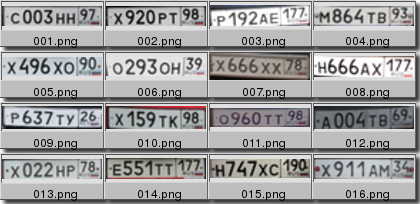
\includegraphics{../presentation/content/out_sr1.png}
  \end{center}
  \caption{Выборка изображений для построения графика для оценки результатов работы алгоритмов по нескольким
  изображениям.}
  \label{fig:samples}
\end{figure}

\begin{figure}[p]
  \centering
  % This file was created by matlab2tikz v0.3.3.
% Copyright (c) 2008--2013, Nico Schlömer <nico.schloemer@gmail.com>
% All rights reserved.
% 
% The latest updates can be retrieved from
%   http://www.mathworks.com/matlabcentral/fileexchange/22022-matlab2tikz
% where you can also make suggestions and rate matlab2tikz.
% 
% 
% 
\begin{tikzpicture}

\begin{axis}[%
width=10cm,
height=7.88709677419355cm,
scale only axis,
xmin=0,
xmax=16,
xlabel={Номер изображения},
ymin=14,
ymax=28,
ylabel={PSNR dB},
legend style={draw=black,fill=white,legend cell align=left}
]
\addplot [
color=blue,
solid
]
table[row sep=crcr]{
1 22.6637207689603\\
2 16.5862621065916\\
3 20.2561814850212\\
4 16.8180326138836\\
5 15.2818944883097\\
6 20.8935173361133\\
7 19.9100975616132\\
8 21.8054095243458\\
9 19.5938529440994\\
10 14.97066690973\\
11 17.6444789637467\\
12 19.6591796988059\\
13 24.5276502442069\\
14 19.6886965973242\\
15 18.0639264824657\\
16 22.7687595823891\\
};
\addlegendentry{Алгоритм с обучаемыми словарями};

\addplot [
color=green!50!black,
dashed
]
table[row sep=crcr]{
1 20.654183811932\\
2 15.5287572495406\\
3 14.6873141103361\\
4 16.906444307724\\
5 16.6431061328363\\
6 15.8814467785726\\
7 15.7004358294634\\
8 20.0170778439843\\
9 15.4643027107035\\
10 16.2470604606123\\
11 17.5627961112945\\
12 23.0775671820967\\
13 22.5057715768468\\
14 17.6125613605738\\
15 17.383467191801\\
16 16.1412027040119\\
};
\addlegendentry{Бикубическая интерполяция};

\end{axis}
\end{tikzpicture}%

  \caption{Результаты алгоритма с тренированными словарями }
  \label{fig:plot_sr1}
\end{figure}

\begin{figure}[p]
  \centering
  % This file was created by matlab2tikz v0.3.3.
% Copyright (c) 2008--2013, Nico Schlömer <nico.schloemer@gmail.com>
% All rights reserved.
% 
% The latest updates can be retrieved from
%   http://www.mathworks.com/matlabcentral/fileexchange/22022-matlab2tikz
% where you can also make suggestions and rate matlab2tikz.
% 
% 
% 
\begin{tikzpicture}

\begin{axis}[%
width=10cm,
height=7.88709677419355cm,
scale only axis,
xmin=0,
xmax=16,
xlabel={Номер изображения},
ymin=12,
ymax=35,
ylabel={PSNR dB},
legend style={draw=black,fill=white,legend cell align=left}
]
\addplot [
color=blue,
solid
]
table[row sep=crcr]{
1 27.4470571608433\\
2 22.8300247931548\\
3 22.1109193658809\\
4 22.0652635937327\\
5 23.6272496813018\\
6 21.6055079117517\\
7 21.4619565703478\\
8 26.9867634881452\\
9 20.9809477047241\\
10 23.2957078121211\\
11 23.9394056382537\\
12 25.5317267141373\\
13 29.2416356490523\\
14 24.1599986234539\\
15 23.7307351145084\\
16 22.5888532577419\\
};
\addlegendentry{Алгоритм с регуляризацией};

\addplot [
color=green!50!black,
solid
]
table[row sep=crcr]{
1 18.4503335459593\\
2 15.9429403769346\\
3 15.9459841548511\\
4 15.5934814518383\\
5 16.9838249182421\\
6 13.7171337206461\\
7 12.7696291928783\\
8 21.6627180369299\\
9 13.6838913514568\\
10 18.8295593160528\\
11 17.4771261841067\\
12 20.0919833166445\\
13 22.2356695114555\\
14 16.697098012576\\
15 18.4542205359683\\
16 15.4386868770896\\
};
\addlegendentry{Начальное приближение};

\end{axis}
\end{tikzpicture}%

  \caption{Результаты работы алгоритма с использование регуляризации \label{plot_sr2}}
\end{figure}

\begin{figure}[p]
  \centering
  % This file was created by matlab2tikz v0.3.3.
% Copyright (c) 2008--2013, Nico Schlömer <nico.schloemer@gmail.com>
% All rights reserved.
% 
% The latest updates can be retrieved from
%   http://www.mathworks.com/matlabcentral/fileexchange/22022-matlab2tikz
% where you can also make suggestions and rate matlab2tikz.
% 
% 
% 
\begin{tikzpicture}

\begin{axis}[%
width=5cm,
height=1cm,
axis on top,
scale only axis,
xmin=0.5,
xmax=50.5,
y dir=reverse,
ymin=0.5,
ymax=10.5,
hide axis,
name=plot1,
title={Начальное приближение}
]
\addplot graphics [xmin=0.5,xmax=50.5,ymin=0.5,ymax=10.5] {../plots/sr2_psnr_rising-1.png};
\end{axis}

\begin{axis}[%
width=5cm,
height=1cm,
axis on top,
scale only axis,
xmin=0.5,
xmax=50.5,
y dir=reverse,
ymin=0.5,
ymax=10.5,
hide axis,
name=plot2,
at=(plot1.below south west),
anchor=above north west,
title={Оригинальное изображение}
]
\addplot graphics [xmin=0.5,xmax=50.5,ymin=0.5,ymax=10.5] {../plots/sr2_psnr_rising-2.png};
\end{axis}

\begin{axis}[%
width=5cm,
height=3.74020102770053cm,
scale only axis,
xmin=0,
xmax=60,
xlabel={Итерация},
ymin=12,
ymax=20,
ylabel={PNSR dB},
name=plot4,
at=(plot2.right of south east),
anchor=left of south west,
title={PSNR}
]
\addplot [
color=blue,
solid,
forget plot
]
table[row sep=crcr]{
1 12.3202813060895\\
2 12.9529644677536\\
3 13.5260641864726\\
4 14.0455567679328\\
5 14.5157791626175\\
6 14.9401084698002\\
7 15.3214501720298\\
8 15.6625515600167\\
9 15.966172416695\\
10 16.2351495750173\\
11 16.4723907826822\\
12 16.6808285374995\\
13 16.8633577505267\\
14 17.022773711704\\
15 17.1617200798005\\
16 17.2826512422842\\
17 17.3878096467359\\
18 17.4792164732515\\
19 17.5586729726292\\
20 17.6277695606153\\
21 17.6878999988837\\
22 17.7402784568312\\
23 17.7859577695793\\
24 17.8258476931939\\
25 17.8607323650764\\
26 17.8912864943554\\
27 17.9180900396926\\
28 17.9416412935904\\
29 17.9623683983446\\
30 17.9806393834473\\
31 17.9967708494893\\
32 18.011035438794\\
33 18.0236682351711\\
34 18.0348722293508\\
35 18.0448229763448\\
36 18.0536725585498\\
37 18.0615529553497\\
38 18.0685789072431\\
39 18.0748503506304\\
40 18.0804544886167\\
41 18.0854675536173\\
42 18.0899563091761\\
43 18.0939793311617\\
44 18.0975881022909\\
45 18.1008279486261\\
46 18.1037388421964\\
};
\end{axis}

\begin{axis}[%
width=5cm,
height=1cm,
axis on top,
scale only axis,
xmin=0.5,
xmax=50.5,
y dir=reverse,
ymin=0.5,
ymax=10.5,
hide axis,
at=(plot4.above north west),
anchor=below south west,
title={Результат}
]
\addplot graphics [xmin=0.5,xmax=50.5,ymin=0.5,ymax=10.5] {../plots/sr2_psnr_rising-3.png};
\end{axis}
\end{tikzpicture}%
  \caption{Пример работы алгоритма с регуляризацией. На графике PSNR хорошо видно, как вырастает PSNR в зависимости
    от шага алгоритма \label{plot_sr2_rising_low}}
\end{figure}

 \begin{figure}[p]
   \centering
   % This file was created by matlab2tikz v0.3.3.
% Copyright (c) 2008--2013, Nico Schlömer <nico.schloemer@gmail.com>
% All rights reserved.
% 
% The latest updates can be retrieved from
%   http://www.mathworks.com/matlabcentral/fileexchange/22022-matlab2tikz
% where you can also make suggestions and rate matlab2tikz.
% 
% 
% 
\begin{tikzpicture}

\begin{axis}[%
width=5cm,
height=0.9cm,
axis on top,
scale only axis,
xmin=0.5,
xmax=100.5,
y dir=reverse,
ymin=0.5,
ymax=18.5,
hide axis,
name=plot1,
title={Начальное приближение}
]
\addplot graphics [xmin=0.5,xmax=100.5,ymin=0.5,ymax=18.5] {../plots/sr2_psnr_rising_2-1.png};
\end{axis}

\begin{axis}[%
width=5cm,
height=0.9cm,
axis on top,
scale only axis,
xmin=0.5,
xmax=100.5,
y dir=reverse,
ymin=0.5,
ymax=18.5,
hide axis,
name=plot2,
at=(plot1.below south west),
anchor=above north west,
title={Оригинальное изображение}
]
\addplot graphics [xmin=0.5,xmax=100.5,ymin=0.5,ymax=18.5] {../plots/sr2_psnr_rising_2-2.png};
\end{axis}

\begin{axis}[%
width=5cm,
height=3.76301826188611cm,
scale only axis,
xmin=0,
xmax=60,
xlabel={Итерация},
ymin=16,
ymax=24,
ylabel={PNSR dB},
name=plot4,
at=(plot2.right of south east),
anchor=left of south west,
title={PSNR}
]
\addplot [
color=blue,
solid,
forget plot
]
table[row sep=crcr]{
1 16.3819645818644\\
2 17.0780369540006\\
3 17.7072119644846\\
4 18.2779056934387\\
5 18.7961056895055\\
6 19.2661449216461\\
7 19.6913393603133\\
8 20.0744644313597\\
9 20.4180785288889\\
10 20.7247161200502\\
11 20.99697867816\\
12 21.2375525901663\\
13 21.4491809002166\\
14 21.6346113256761\\
15 21.7965374526836\\
16 21.9375443813036\\
17 22.0600651225625\\
18 22.1663501942838\\
19 22.2584502336536\\
20 22.3382099167395\\
21 22.4072708002286\\
22 22.4670806035736\\
23 22.5189066898221\\
24 22.5638518996966\\
25 22.6028713265497\\
26 22.6367890211028\\
27 22.6663139523695\\
28 22.6920548161245\\
29 22.7145334789205\\
30 22.7341969841924\\
31 22.7514281393378\\
32 22.7665547601366\\
33 22.7798576811311\\
34 22.7915776553607\\
35 22.8019212700101\\
36 22.8110660003991\\
37 22.8191645163655\\
38 22.8263483445616\\
39 22.8327309788807\\
40 22.8384105200143\\
41 22.8434719145521\\
42 22.8479888543236\\
43 22.8520253879912\\
44 22.8556372892352\\
45 22.8588732191953\\
46 22.8617757150688\\
47 22.864382031827\\
48 22.8667248597992\\
};
\end{axis}

\begin{axis}[%
width=5cm,
height=0.9cm,
axis on top,
scale only axis,
xmin=0.5,
xmax=100.5,
y dir=reverse,
ymin=0.5,
ymax=18.5,
hide axis,
at=(plot4.above north west),
anchor=below south west,
title={Результат}
]
\addplot graphics [xmin=0.5,xmax=100.5,ymin=0.5,ymax=18.5] {../plots/sr2_psnr_rising_2-3.png};
\end{axis}
\end{tikzpicture}%
   \caption{Пример изображений алгоритма с регуляризацией для изображения с более высоким исходным разрешением.
     \label{plot_sr2_rising_high}}
 \end{figure}


\subsection{Средства}
Работа по подготовке изображений, построению графиков, реализации алгоритмов была выполнена в среде MatLab. Полный
исходный код можно найти по адресу \url{https://github.com/ulex/sr-license-plates}.


% \subsection{Дальнейшее исследование}
% В дальнейшем планируется использовать

\subsection{Вывод}
В результате опытов было установлено, что исследуемые алгоритмы применимы к задаче повышения разрешения изображений
автомобильных номеров. Результаты работы могут быть использованы при выборе алгоритма для этой задачи.
% Была проделана следующая работа:
% \begin{itemize}
%   \item Исследованы современные подходы к задаче SR.
%   \item Реализован алгоритм повышения разрешения с использованием регуляризации.
%   \item Проведено исследование по качеству восстановления изображение
% \end{itemize}<++>

\newpage
\nocite{*}
\bibliographystyle{unsrt}
\bibliography{bib}

